\chapter{LITERATURE REVIEW}
\pagebreak

\begin{center}
{\LARGE\textbf{LITERATURE REVIEW}}
\end{center}

\section{Introduction}
Here is an example of one figure introduction introduction introduction introduction introduction introduction introduction introduction introduction introduction introduction introduction introduction introduction introduction introduction introduction introduction introduction introduction introduction introduction introduction introduction introduction introduction introduction introduction introduction introduction introduction introduction introduction introduction introduction introduction introduction introduction introduction introduction introduction introduction introduction introduction introduction introduction introduction introduction introduction introduction introduction introduction introduction introduction introduction introduction introduction introduction introduction introduction introduction introduction introduction introduction as in Figure~\ref{f11}


\begin{figure}[ht]
\begin{center}
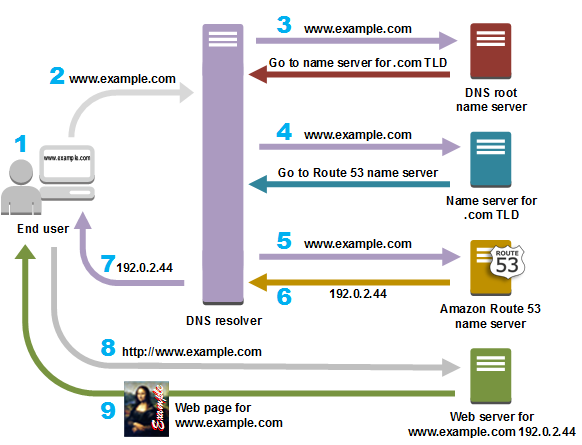
\includegraphics[width=0.6\textwidth]{figures/samples/Fig1.png}
\caption{This is figure 1 in chapter 3}
\label{f11}
\end{center}
\end{figure}

introduction introduction introduction introduction introduction introduction introduction introduction introduction introduction introduction introduction introduction introduction introduction introduction introduction introduction introduction introduction introduction introduction introduction introduction introduction introduction introduction introduction introduction introduction introduction introduction introduction introduction introduction introduction introduction introduction introduction introduction introduction introduction Here is an example of one figure (Figure~\ref{fig:test}) that divided into two sub figures as Figure~\ref{fig:sub1}, Figure~\ref{fig:sub2}, Figure~\ref{fig:sub3}.

\begin{figure}[ht]
\centering
    \begin{subfigure}{.3\textwidth}
         \centering
          
\includegraphics[width=.8\linewidth]{figures/samples/it.png}
           \caption{Machine Learning methods}
        \label{fig:sub1}
        \end{subfigure}%
    \begin{subfigure}{.3\textwidth}
         \centering
        
\includegraphics[width=.8\linewidth]{figures/samples/it.png}
        \caption{Deep learning methods}
        \label{fig:sub2}
        \end{subfigure}
            \begin{subfigure}{.3\textwidth}
         \centering
        
\includegraphics[width=.8\linewidth]{figures/samples/it.png}
        \caption{Recurrent neural networks}
        \label{fig:sub3}
        \end{subfigure}
        \caption{Artificial Intelligent}
\label{fig:test}
\end{figure}

\subsection{Introduction}
Here is an example of one figure
\subsubsection{Introduction}
Here is an example of one figureintroduction introduction introduction introduction introduction introduction introduction introduction introduction introduction introduction introductionintroduction introduction introduction introduction introduction introduction introduction introduction introduction introduction introduction introductionintroduction introduction introduction introduction introduction introduction introduction introduction introduction introduction introduction introductionintroduction introduction introduction introduction introduction introduction introduction introduction introduction introduction introduction introductionintroduction introduction introduction introduction introduction introduction introduction introduction introduction introduction introduction introductionintroduction introduction introduction introduction introduction introduction introduction introduction introduction introduction introduction introductionintroduction introduction introduction introduction introduction introduction introduction introduction introduction introduction introduction introductionintroduction introduction introduction introduction introduction introduction introduction introduction introduction introduction introduction introduction
Here is another example for putting two small figure side by side as in Figure~\ref{fig:test1}, Figure~\ref{fig:test2}.

\begin{figure}[ht]
\centering
\begin{minipage}{.5\textwidth}
  \centering
  
\includegraphics[width=.9\linewidth]{figures/samples/it.png}
  \captionof{figure}{A figure}
  \label{fig:test1}
\end{minipage}%
\begin{minipage}{.5\textwidth}
  \centering
  
\includegraphics[width=.9\linewidth]{figures/samples/it.png}
  \captionof{figure}{Another figure}
  \label{fig:test2}
\end{minipage}
\end{figure}


 introduction introduction introduction introduction ~\cite{ref1} in Figure~\ref{fig1}. introduction introduction introduction introduction introduction introduction introduction introduction introduction introduction introduction introduction introduction introduction introduction introduction introduction ~\cite{ref2}. introduction introduction introduction as in Figure~\ref{fig2} introduction introduction introduction introduction introduction introduction introduction introduction introduction introduction introduction introduction introduction introduction introduction introduction introduction introduction introduction introduction 
~\cite{ref3},\cite{ref4}. 



\begin{figure}[ht]
\begin{center}

\includegraphics[width=0.6\textwidth]{figures/samples/it.png}
\caption{Dummy figure 2}
\label{fig1}
\end{center}
\end{figure}

\begin{sidewaysfigure}[ht]
\begin{center}

\includegraphics[width=0.6\textwidth]{figures/samples/qu.png}
\caption{The image of the introduction}
\label{fig2}
\end{center}
\end{sidewaysfigure}

\hfill \break
\hfill \break
\hfill \break
\hfill \break
\hfill \break
\hfill \break
\hfill \break
\hfill \break
\hfill \break
\hfill \break
\hfill \break
\hfill \break
\hfill \break
\hfill \break
\hfill \break
\hfill \break
\hfill \break

\section{Background}
Introduction introduction introduction introduction introduction introduction introduction introduction introduction introduction introduction introduction introduction introduction introduction introduction introduction introduction introduction introduction introduction introduction introduction introduction introduction introduction introduction introduction introduction introduction \cite{ref1}. 
      

introduction introduction introduction introduction introduction introduction introduction introduction introduction introduction introduction introduction introduction introduction introduction introduction introduction \cite{ref2}. introduction introduction introduction introduction introduction introduction introduction introduction introduction introduction introduction introduction introduction introduction introduction introduction introduction introduction introduction introduction introduction introduction introduction introduction introduction introduction introduction introduction introduction introduction introduction introduction introduction introduction introduction introduction introduction introduction 
\cite{ref5},\cite{ref6}. as shown in eq. (\ref{eq1})

\begin{equation}
Z=\sqrt{X^{2}+Y^{2}}  
\label{eq1}
\end{equation}


Table~\ref{tab1}, Table~\ref{tab2}, Table~\ref{tab3} shows the database for Engineering in different ways


\begin{table}[ht]
\caption{Comparison between related works}
\begin{center}
\begin{tabular}{lllll}
\hline
Name & Method & Ref & Year & Idea                                           \\ \hline

\includegraphics[width=0.2\textwidth, height=30mm]{figures/samples/it.png}   & CNN    & 1   & 2020 &  Dina \\

\includegraphics[width=0.2\textwidth, height=30mm]{figures/samples/it.png}  & RNN    & 2   & 2020 & Mona \\
Dina & CNN    & 1   & 2020 & 
\includegraphics[width=0.2\textwidth, height=20mm]{figures/samples/qu.png} \\
Mona & RNN    & 2   & 2020 &  
\includegraphics[width=0.2\textwidth, height=20mm]{figures/samples/qu.png} \\ \hline
\end{tabular}
    \end{center}
\label{tab1}
\end{table}

\begin{figure}[ht]
\begin{center}

\includegraphics[width=0.1\textwidth]{figures/samples/it.png}
\caption{Dummy figure 2}
\label{fig6}
\end{center}
\end{figure}

\begin{table}[ht]
\caption{Comparison between Wired and wireless networks}
\begin{center}
{\small
%\begin{tabular}{lll}
\begin{tabular}{p{.2\textwidth}p{.2\textwidth}p{.4\textwidth}}

\hline
Specifications       & Wired network    & Wireless network       \\ \hline
Speed of operation   & Higher           & lower compare to wired networks, But advanced wireless technologies such as LTE, LTE-A and WLAN-11ad will make it possible to achieve speed par equivalent to wired network \\
System Bandwidth     & High              & Low, as Frequency Spectrum is very scarse resource    \\
Cost                 & Less as cables are not expensive      & More as wireless subscriber stations, wireless routers, wireless access points and adapters are expensive                 \\
Installation         & Wired network installation is cumbersome and it requires more time   & Wireless network installation is easy and it requires less time             \\
Mobility            & Limited, as it operates in the area covered by connected systems with the wired network                & Not limited, as it operates in the entire wireless network coverage         \\
Transmission medium     & copper wires, optical fiber cables, ethernet   & EM waves or radiowaves or infrared  \\
Network coverage extension    & requires hubs and switches for network coverage limit extension  & More area is covered by wireless base stations which are connected to one another.    \\
Applications           & LAN (Ethernet), MAN        & WLAN, WPAN(Zigbee, bluetooth), Infrared, Cellular(GSM,CDMA, LTE) \\
Channel Interference and signal power loss & Interference is less as one wired network will not affect the other                          & Interference is higher due to obstacles between wireless transmitter and receiver e.g. weather conditions, reflection from walls, etc.                                      \\
QoS (Quality of Service)                   & Better           & Poor due to high value of jitter and delay in connection setup  \\
Reliability           & High compare to wireless counterpart, as manufactured cables have higher performance due to existence of wired technology since years. & Reasonably high, This is due to failure of router will affect the entire network.  \\ \hline
\end{tabular}
}
    \end{center}
\label{tab2}
\end{table}

%\begin{table}[ht]
\begin{sidewaystable}[ht]
\caption{Comparison between Wired and wireless networks}
\begin{center}

\begin{tabular}{p{.2\textwidth}p{.3\textwidth}p{.4\textwidth}}
\hline
Specifications       & Wired network    & Wireless network       \\ \hline
Speed of operation   & Higher           & lower compare to wired networks, But advanced wireless technologies such as LTE, LTE-A and WLAN-11ad will make it possible to achieve speed par equivalent to wired network \\
System Bandwidth     & High              & Low, as Frequency Spectrum is very scarse resource    \\
Cost                 & Less as cables are not expensive      & More as wireless subscriber stations, wireless routers, wireless access points and adapters are expensive                 \\
Installation         & Wired network installation is cumbersome and it requires more time   & Wireless network installation is easy and it requires less time             \\
Mobility            & Limited, as it operates in the area covered by connected systems with the wired network                & Not limited, as it operates in the entire wireless network coverage         \\
Transmission medium     & copper wires, optical fiber cables, ethernet   & EM waves or radiowaves or infrared  \\
Network coverage extension    & requires hubs and switches for network coverage limit extension  & More area is covered by wireless base stations which are connected to one another.    \\
Applications           & LAN (Ethernet), MAN        & WLAN, WPAN(Zigbee, bluetooth), Infrared, Cellular(GSM,CDMA, LTE) \\
Channel Interference and signal power loss & Interference is less as one wired network will not affect the other                          & Interference is higher due to obstacles between wireless transmitter and receiver e.g. weather conditions, reflection from walls, etc.                                      \\
QoS (Quality of Service)                   & Better           & Poor due to high value of jitter and delay in connection setup  \\
Reliability           & High compare to wireless counterpart, as manufactured cables have higher performance due to existence of wired technology since years. & Reasonably high, This is due to failure of router will affect the entire network.    \\ \hline
\end{tabular}

    \end{center}
\label{tab3}
\end{sidewaystable}
%\end{table}

\begin{itemize}     
	\item[$-$] Chapter 1      
	\item[$\square$] Chapter 2     
	 \item Chapter 3       
\end{itemize}

\begin{enumerate}
  \item The labels consists of sequential numbers.
  \item The numbers starts at 1 with every call to the enumerate environment.
\end{enumerate}

\begin{enumerate}
\item The first point
\item the second point
\item the third point
\end{enumerate}

\begin{table}[h]
\caption{Course grades}
\begin{center}
\begin{tabular}{llll}
\hline
Day      & Course Title      & Grade & Level \\ \hline
Saturday & Operating System  & A     & 5     \\ \hline
Sunday   & Data Structure    & B     & 4     \\ \hline
Monday   & Computer Networks & A     & 7     \\ \hline
\end{tabular}
\end{center}
\label{Tab4}
\end{table}